% This is samplepaper.tex, a sample chapter demonstrating the
% LLNCS macro package for Springer Computer Science proceedings;
% Version 2.20 of 2017/10/04
%
\documentclass[runningheads]{llncs}
%
\usepackage{graphicx}
\usepackage{multirow}
\usepackage{hyperref}
\hypersetup{
    colorlinks=true,
    linkcolor=blue,
    urlcolor=blue,
}
% \usepackage[numbers]{natbib}
% \bibliographystyle{plainnat}

% \usepackage{amsmath}

% Used for displaying a sample figure. If possible, figure files should
% be included in EPS format.
\begin{document}
% If you use the hyperref package, please uncomment the following line
% to display URLs in blue roman font according to Springer's eBook style:
% \renewcommand\UrlFont{\color{blue}\rmfamily}

% \title{Contribution Title\thanks{Supported by organization x.}}
\title{Deep Learning Approaches for Intracranial Hemorrhage Sub-Type Classification
\thanks{Project for CMPUT 617: Medical Image Analysis. Fall 2019. University of Alberta.}}
%
\titlerunning{DL Approaches for ICH Sub-Type Classification}
% If the paper title is too long for the running head, you can set
% an abbreviated paper title here
%
\author{Alexander William Wong\orcidID{0000-0002-9773-7484}}
%
\authorrunning{A. Wong}

% First names are abbreviated in the running head.
% If there are more than two authors, 'et al.' is used.
%
\institute{University of Alberta, Edmonton AB, Canada\\
\email{\href{mailto:alex.wong@ualberta.ca}{alex.wong@ualberta.ca}}
% \url{http://www.springer.com/gp/computer-science/lncs} \and
% ABC Institute, Rupert-Karls-University Heidelberg, Heidelberg, Germany\\
% \email{\{abc,lncs\}@uni-heidelberg.de}
}
%
\maketitle % typeset the header of the contributions
\begin{abstract}
This work applies deep learning approaches for predicting sub-categories of intracranial hemorrhages from brain computed topography scans.
An intracranial hemorrhage, defined as internal bleeding within the skull, is a severe medical emergency requiring immediate and often invasive treatment.
We provide a comprehensive overview for preprocessing cranial CT scans and explore multiple architectures for this classification experiment.
Finally, we summarize the different approaches used by the top Kaggle RSNA Intracranial Hemorrhage Detection competition submissions.
Our source code, models, and submission files are available at \href{https://github.com/awwong1/rsna-hemorrhage-classification}{github.com/awwong1/rsna-hemorrhage-classification}.

\keywords{Medical Image Analysis \and Intracranial Hemorrhage}
\end{abstract}
%
%
%
\section{Introduction}

Intracranial hemorrhage (ICH), when bleeding occurs in the cranium, is a severe medical emergency caused by physical trauma (head injury), non-traumatic cases (stroke, aneurysm), or disorders with blood clotting.
Blood pools within the skull resulting in increased intracranial pressure which can irreversibly cause brain damage.
In severe cases brain herniation, where parts of the brain are squeezed past the structures in the skull, may occur.
To maximize survival probability, it is critical that physicians quickly recognize and treat the various types of ICH.

Diagnosing ICH is an often time consuming procedure involving coordination between multiple specialists~\cite{PMID:9537967}.
First, a radiology technologist performs a computed topography (CT) scan to visualize the contents of the skull.
Neurologists then review the scans of the cranium to find the position and type of ICH before proceeding with further therapy.
Our work proposes an algorithm which takes as input a 2D slice of a CT scan and detects five different sub-categories of ICH, as specified by the RSNA Intracranial Hemorrhage Detection dataset~\cite{kaggle/rsna-ich}.

\section{Background}

\subsection{Task Overview}

\begin{figure}[htbp]
    \centering
    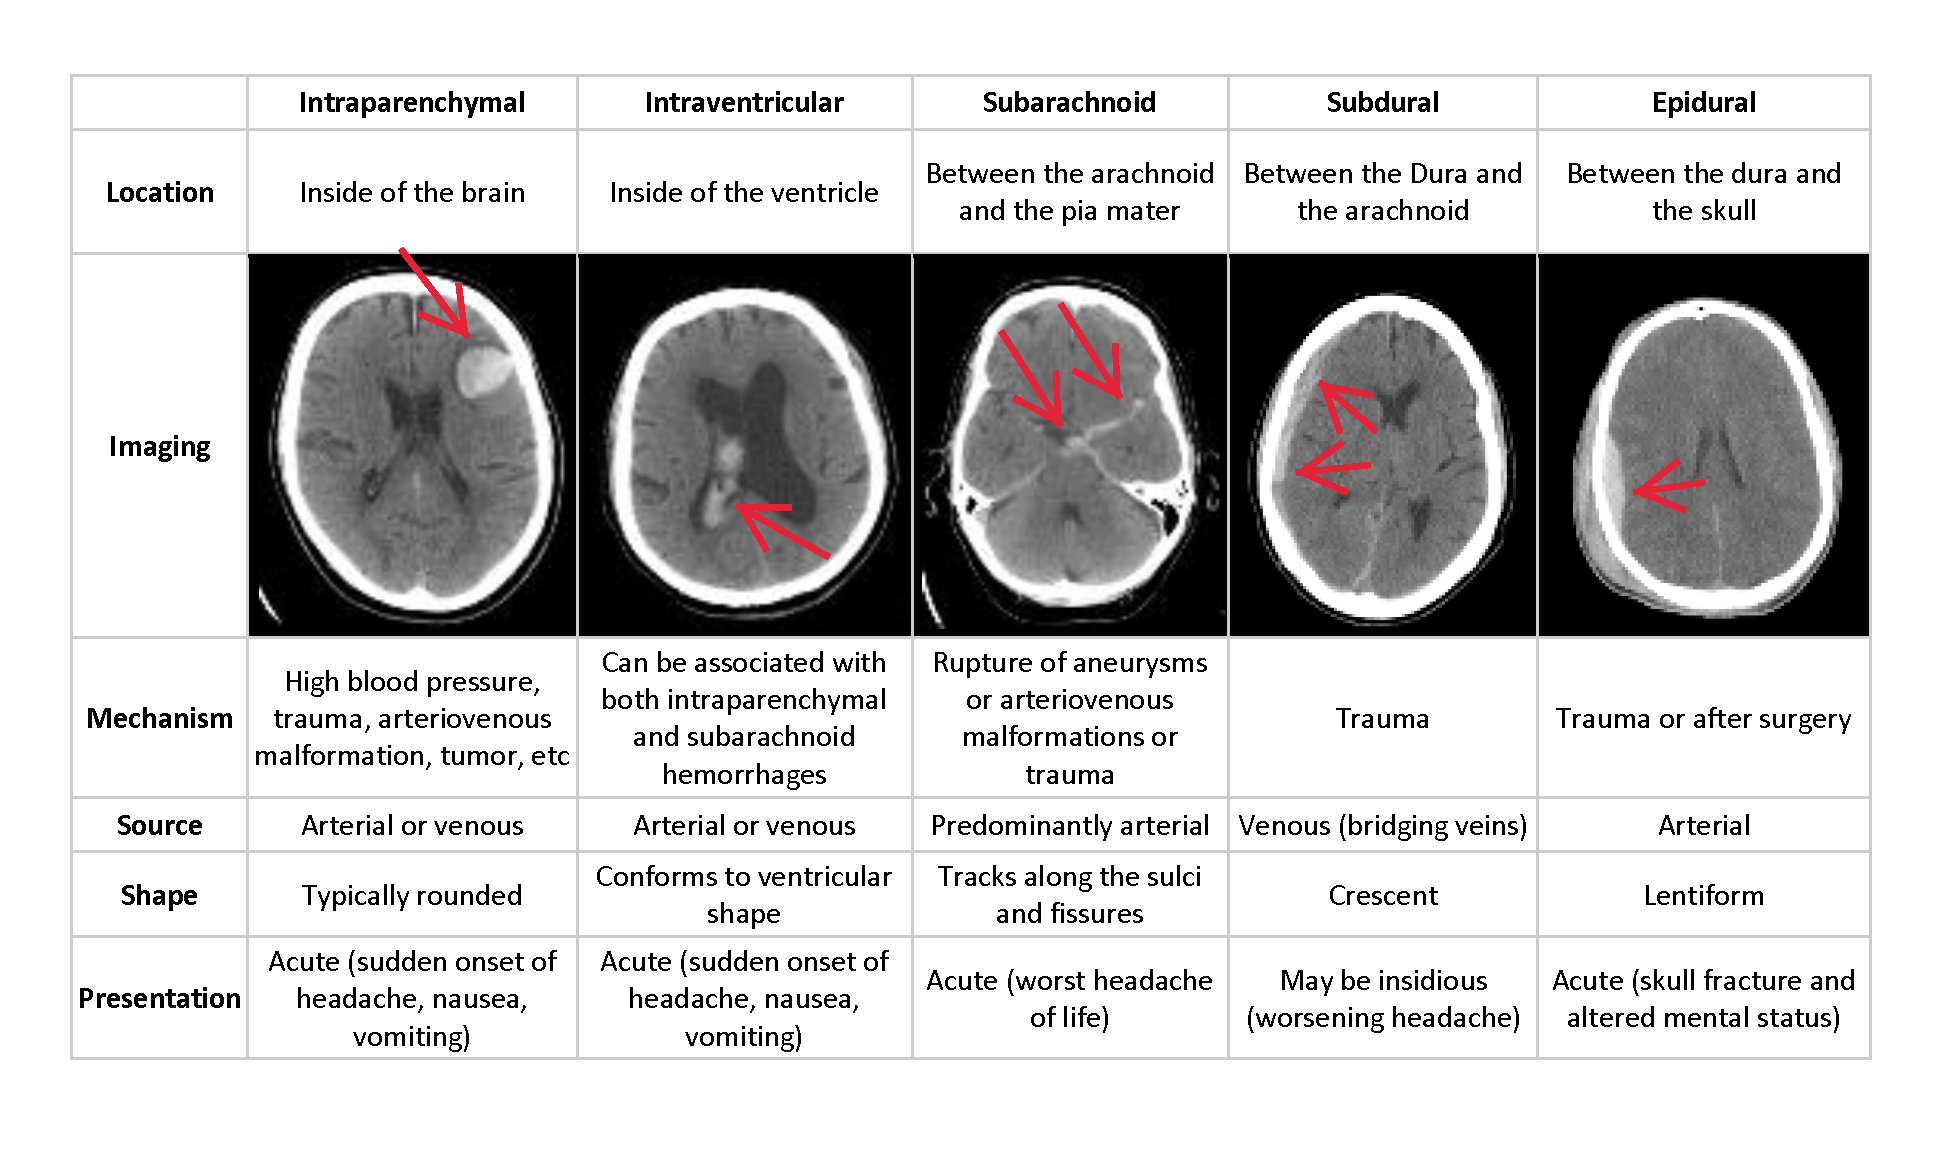
\includegraphics[width=4.8in]{fig/subtypes-of-hemorrhage}
    \caption{Classification samples: five subtypes of intracranial hemorrhages with corresponding characteristics including mechanism, source, shape, and patient symptoms.}
    \label{fig:ich-subtypes}
\end{figure}

Our task is to detect the probability of five different variants of ICH existing within a CT scan of a human head: intraparenchymal, intraventricular, subarachnoid, subdural, and epidural.
A summary of the five ICH subtypes can be found in Fig.~\ref{fig:ich-subtypes} with corresponding CT scan examples\footnote{Image source: \href{https://www.kaggle.com/marcovasquez/basic-eda-data-visualization\#1--What-is-an-intracranial-hemorrhage}{kaggle.com/marcovasquez/basic-eda-data-visualization}}.

\begin{description}
    \item [Intraparenchymal hemorrhage] is characterized by bleeding within the brain parenchyma, or the functional substance composing the brain itself~\cite{10.1001/jama.2019.2413}. These hemorrhages are typically round in shape.
    \item [Intraventricular hemorrhage] is where the bleeding occurs in the brain's ventricular system where the cerebrospinal fluid is produced~\cite{PMID:20425231}. Visually, this hemorrhage appears in the dark center of the brain.
    \item [Subarachnoid hemorrhage] is when bleeding is released into the space surrounding the brain~\cite{ABRAHAM2016901}. The primary visual characteristic separating subarachnoid and intraparenchymal hemorrhages are the tendril like tracks occurring along the fissures of the brain.
    \item [Subdural hematoma] is the bleeding between the inner layer of the of the dura mater and the arachnoid mater~\cite{PMID:28558815}. This hemorrhage occurs in the intermediary membranes that surround the brain. The pooled blood is typically not in direct contact with the skull or brain parenchyma.
    \item [Epidural hematoma] is when bleeding occurs between the outer membrane covering the brain (dura mater) and the skull~\cite{ISBN:9780199710041}. One distinction between subdural and epidural hematomas are that epidural hematomas are typically oval/lens shaped, while the subdural hematomas are crescent shaped.
\end{description}

\subsection{Kaggle Challenge Data Overview}

The CT scans provided by Kaggle are stored as Digital Imaging and Communications in Medicine (DICOM) files, an international standard for the representation, exchange, and communication of digital medical images~\cite{mildenberger2002introduction}.
A summary of the Kaggle \texttt{stage\_2} challenge data is provided in Tab.~\ref{tab:data_overview}.

\begin{table}[htbp]
    \centering
    \tabcolsep=0.21cm
    \caption{RSNA Intracranial Hemorrhage Detection Stage 2 file summary.}
    \label{tab:data_overview}
    \begin{tabular}{|c|c|c|}
        \hline
        Dataset & \# DICOM Files & Size (GiB) \\ \hline
        Train + Validation & 752,803 & 370.48 \\ 
        Test    & 121,232 & 59.66 \\ \hline
    \end{tabular}
\end{table}

All DICOM files in the training data are labeled with a \texttt{1} or \texttt{0} for each of the five ICH subtypes, with an additional \texttt{any} label indicating the presence of one or more ICH classifications.
As shown in Tab.~\ref{tab:train_by_count}, a single DICOM file may have more than one ICH classification.
The test dataset is used for the Kaggle competition submission and therefore the ground truth labels are not provided.

\begin{table}[htbp]
    \centering
    \caption{ICH Stage 2 training data summary by sub-type and by ICH count per DICOM file. The \texttt{pos\_weight} is the count of negative divided by positive samples.}
    \label{tab:train_by_count}

    \begin{minipage}{.49\linewidth}
        \centering
        \tabcolsep=0.1cm
        \begin{tabular}{|c|c|c|}
            \hline
            Sub-Type Label & \# Files & \texttt{pos\_weight} \\ \hline
            Epidural & 3,145 & 238.37 \\
            Intraparenchymal &  36,118 & 19.84 \\
            Intraventricular &  26,205 & 27.73 \\
            Subarachnoid & 35,675 & 20.10 \\
            Subdural & 47,166 & 14.96 \\
            Any & 107,933 & 5.97 \\ \hline
            % None (No ICH) & 644,870 \\ \hline
        \end{tabular}
    \end{minipage}
    \begin{minipage}{.49\linewidth}
        \centering
        \tabcolsep=0.21cm
        \begin{tabular}{|c|c|}
            \hline
            \# ICH & \# Files \\ \hline
            1 & 75,859 \\
            2 & 24,826 \\
            3 &  6,217 \\
            4 &  1,008 \\
            5 &     23 \\
            0 & 644,870 \\ \hline
        \end{tabular}
    \end{minipage}
\end{table}

Each DICOM file contained a set of related meta tags storing additional information about the patient and study associated with the CT scan.
% A sample set of meta tags and values can be found in Tab.~\ref{tab:sample_dicom_meta}.
For our experiment, we utilized the raw pixel data, the rescale intercept, rescale slope, window center, and window width.
The raw pixel data was represented in a $512 \times 512$ matrix with values spanning the entire 16 bit signed integer space, ranging from -32,768 to 32,767.

% \begin{table}[htbp]
%     \centering
%     \caption{DICOM Meta tags and values contained in ID\_051688a0d.dcm.}
%     \label{tab:sample_dicom_meta}
%     \begin{tabular}{|c|l|c|l|}
%         \hline
%         Key ID & Key Readable & Type & Meta Value \\ \hline
%         (0008, 0018) & SOP Instance UID                    & UI & ID\_051688a0d \\
%         (0008, 0060) & Modality                            & CS & 'CT' \\
%         (0010, 0020) & Patient ID                          & LO & 'ID\_b5d9e9e1' \\
%         (0020, 000d) & Study Instance UID                  & UI & ID\_65adb6c01d \\
%         (0020, 000e) & Series Instance UID                 & UI & ID\_5e5b435537 \\
%         (0020, 0010) & Study ID                            & SH & '' \\
%         (0020, 0032) & Image Position (Patient)            & DS & ['-125.000', '-113.458', '57.150'] \\
%         \multirow{2}{*}{(0020, 0037)} & \multirow{2}{*}{Image Orientation (Patient)} & \multirow{2}{*}{DS} & ['1.0', '0.0', '0.0', '0.0', \\
%         & & & \multicolumn{1}{r|}{'0.961262', '-0.275637']} \\
%         (0028, 0002) & Samples per Pixel                   & US & 1 \\
%         (0028, 0004) & Photometric Interpretation          & CS & 'MONOCHROME2' \\
%         (0028, 0010) & Rows                                & US & 512 \\
%         (0028, 0011) & Columns                             & US & 512 \\
%         (0028, 0030) & Pixel Spacing                       & DS & ['0.488281', '0.488281'] \\
%         (0028, 0100) & Bits Allocated                      & US & 16 \\
%         (0028, 0101) & Bits Stored                         & US & 16 \\
%         (0028, 0102) & High Bit                            & US & 15 \\
%         (0028, 0103) & Pixel Representation                & US & 1 \\
%         (0028, 1050) & Window Center                       & DS & "40" \\
%         (0028, 1051) & Window Width                        & DS & "150" \\
%         (0028, 1052) & Rescale Intercept                   & DS & "-1024" \\
%         (0028, 1053) & Rescale Slope                       & DS & "1" \\
%         (7fe0, 0010) & Pixel Data                          & OW & Array of 524288 elements \\
%         \hline
%     \end{tabular}
% \end{table}

\subsection{Literature Survey}
Brain CT scan analysis is an emerging domain of research in the medical computer vision community~\cite{10.1007/978-3-319-24574-4_28,10.1007/978-3-030-11723-8_46,10.1038/s41551-018-0324-9,lee2018practical}.
One popular architecture for biomedical image segmentation is U-Net, originally applied to the problem of brain tumor segmentation from 2D CT scans~\cite{10.1007/978-3-319-24574-4_28}.
In~\cite{10.1007/978-3-030-11723-8_46}, a deep learning approach for ICH segmentation in 3D CT scan volumes is presented with dice accuracy comparable to radiologists.
An explainable deep-learning algorithm to detect ICH in small datasets is provided in~\cite{10.1038/s41551-018-0324-9}, accelerating physician confidence for adopting deep-learning systems into practice.
Work from~\cite{lee2018practical} showcased a deep learning window setting optimization module for determining appropriate CT scan windowing parameters to determine ICH and urinary stones, rather than relying on expert human knowledge.

\section{Methodology}

\subsection{Data Pre-processing}

The raw pixel data provided in the DICOM scans required additional processing to enhance the different characteristics of the human head.
Windowing, or grey-level mapping, is a contrast enhancing technique used by radiologists to change the appearance of a CT scan to emphasize different structures~\cite{TIDWELL199965}.
A conversion into the Hounsfield scale, which reduced the maximum and minimum range of the raw pixel values, is required before the windowing is applied~\cite{DEVOS2009609}.

\begin{figure}[htbp]
    \centering
    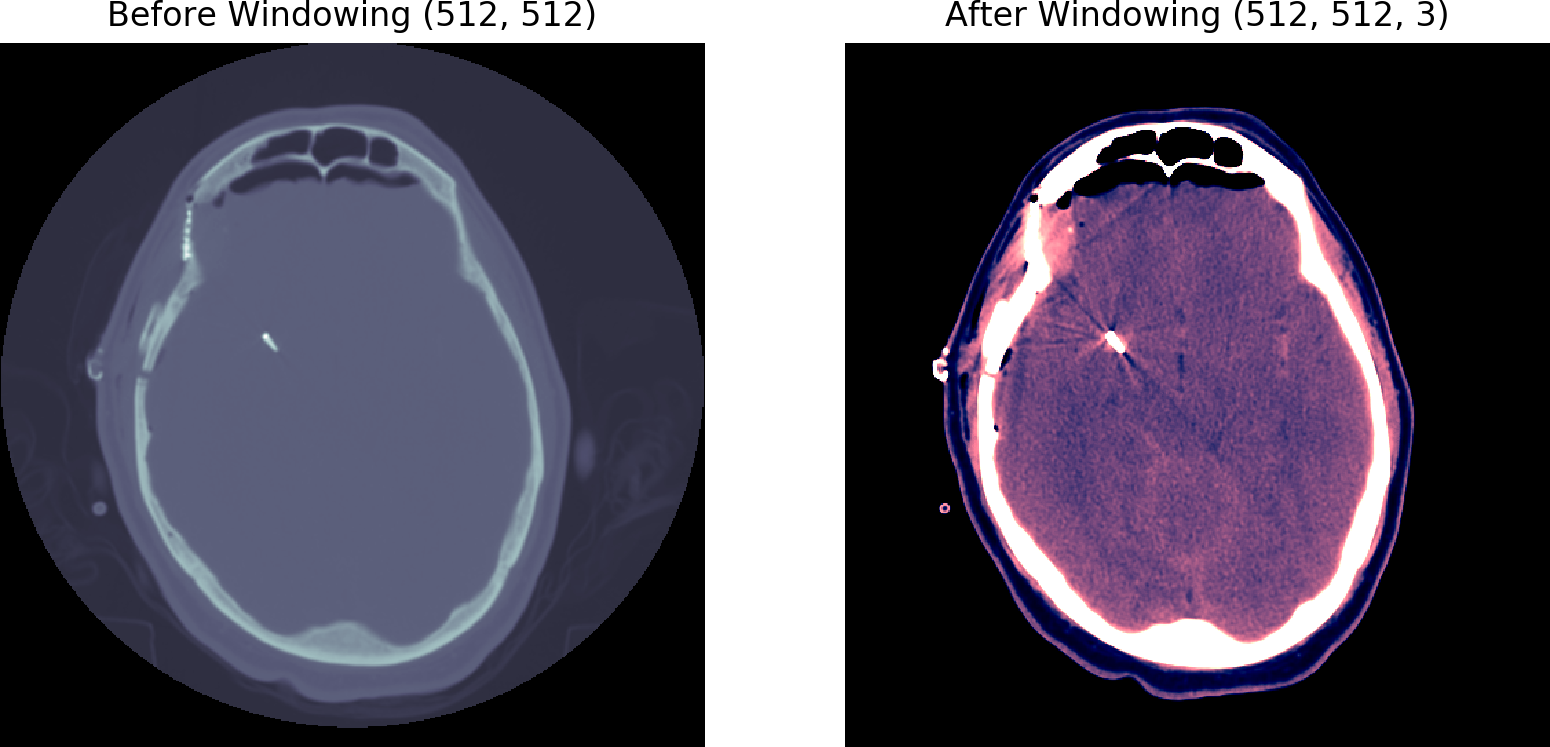
\includegraphics[width=4.8in]{fig/dicom_window}
    \caption{ID\_051688a0d: Left, grey scale raw pixel values; right, three channel brain, subdural, and soft tissue windowing displayed with \texttt{matplotlib.cm.bone} color map. The scan was labeled as having a subarachnoid and subdural intracranial hemorrhage.}
    \label{fig:dicom_windowing}
\end{figure}

We converted the single channel, grey scale pixel data into a three channel image where channels represented the brain window, the subdural (blood) window, and the soft tissues window.
The reference window values used were taken from~\cite{radiopaedia/windowing}, where brain was centered 40 with a width of 80, subdural was centered 80 with a width of 200, and soft tissues was centered 40 with a width of 380.
A sample CT scan, with the multiple window transformations and concatenated three channel image, can be found in Fig.~\ref{fig:dicom_windowing}.

The windowed characteristics of the cranium are emphasized in Fig.~\ref{fig:dicom_windowing_breakdown}.
The subdural channel revealed a mass near the top left of the image, indicating the pooled blood/subdural hematoma.
Without the image processing, the presence of the pooled blood would be difficult to distinguish from the rest of the image.

\begin{figure}[htbp]
    \centering
    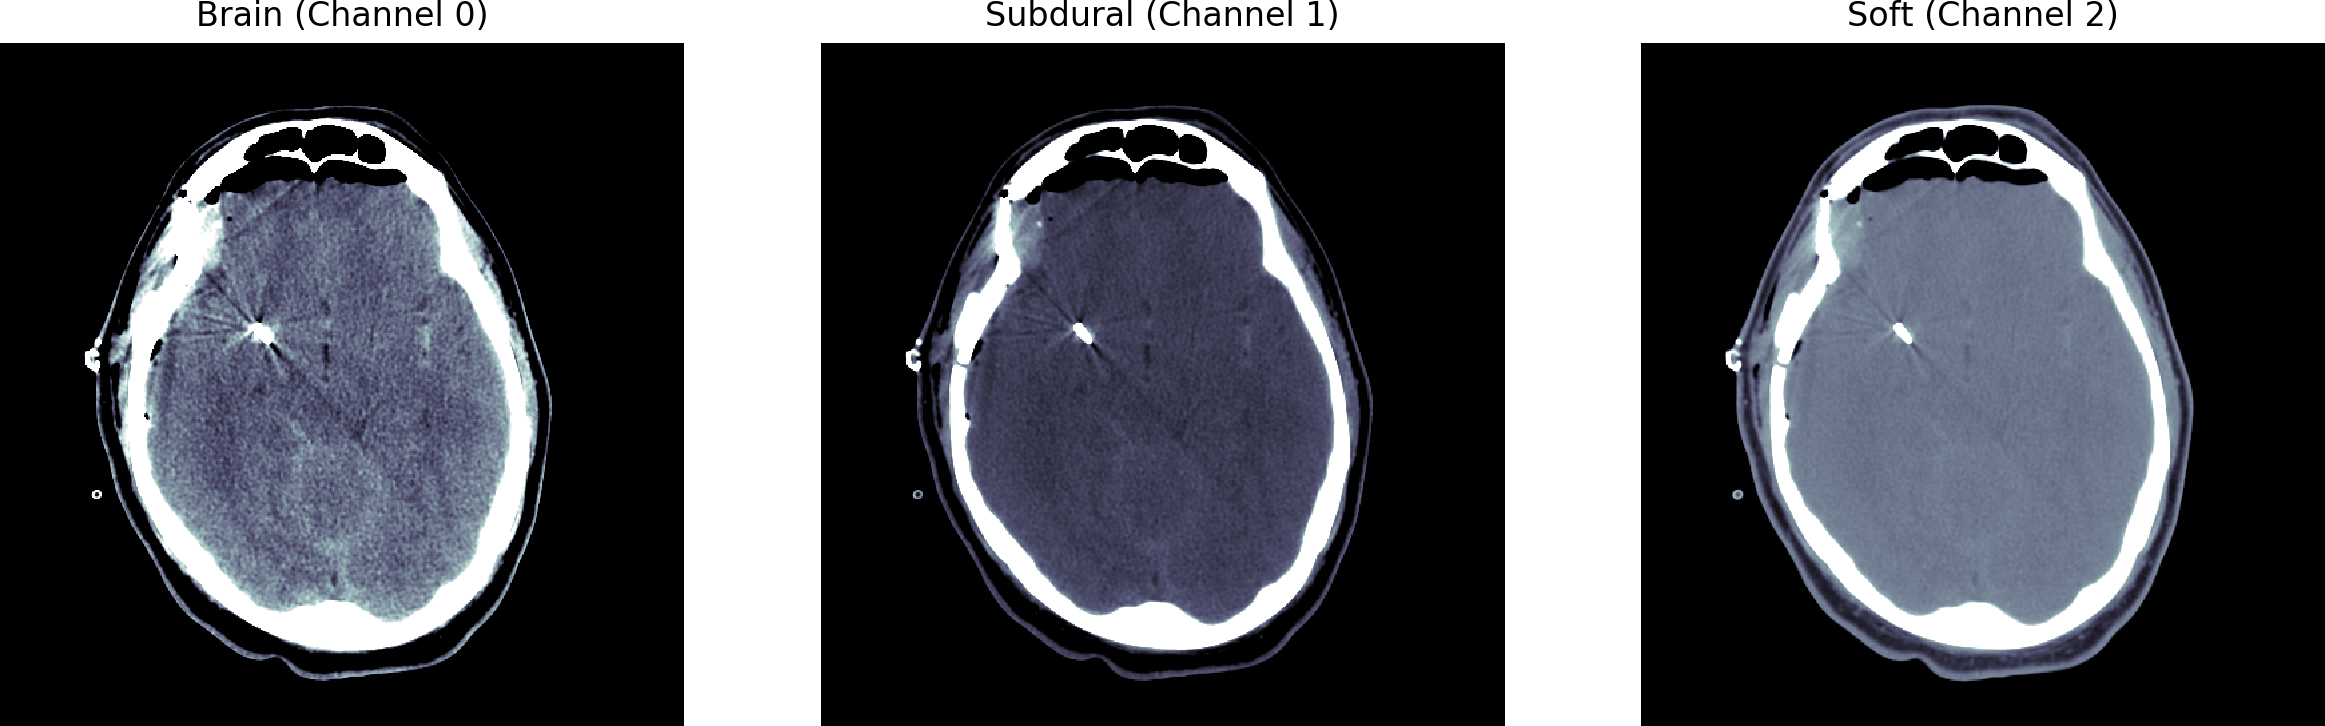
\includegraphics[width=4.8in]{fig/dicom_channels}
    \caption{ID\_051688a0d: Isolated brain, subdural, and soft tissue windowing results.}
    \label{fig:dicom_windowing_breakdown}
\end{figure}

\subsection{Model Architecture and Training}

We approach this task as a typical image classification problem using the popular ResNet family of model architectures~\cite{He_2016_CVPR}.
We first initialized our models with pretrained weights from the ILSVRC 2012 image classification challenge~\cite{ILSVRC15}.
To adhere to our classification task, the final linear layer was modified to output 6 values.
We used the Binary Cross Entropy with Logits Loss (\texttt{BCEWithLogitsLoss}).
For our training optimizer, we used Adam with a learning rate of $2*10^{-5}$ and trained our models for 5 epochs.
We used the \texttt{NVIDIA/apex}\footnote{PyTorch mixed precision and acceleration extension: \href{https://github.com/NVIDIA/apex}{github.com/NVIDIA/apex}} PyTorch extension with optimization level \texttt{"O1"} for automatic mixed precision support and GPU acceleration during training.

For both training and evaluation, we resized the images to be 224 by 224 pixels.
In addition, we applied a random shift scale rotate transformation (rotation limit of 14 degrees), and a random horizontal flip ($p=0.5$) to the training dataset.
For local model parameter/architecture search, we split the provided labelled data into a 95\% train and 5\% validation dataset using the \texttt{random\_split} method.
To evaluate the effect of weighting the positive label losses relative to its sparse representation within the dataset we reran the experiments, setting our loss \texttt{pos\_weight} parameter to $\frac{\# Neg}{\# Pos}$ for each of the 6 labels.

For each architecture ResNet-34, ResNet-50 and ResNet-101, we repeated the training process three times to determine the final Kaggle submission model parameters.
To generate the Kaggle submission files, we resumed training using the parameters from the model with the lowest validation loss.
We fine tuned over the entire labelled dataset for an additional 1 epochs with a learning rate of $1*10^{-5}$ before performing inference over the unlabelled test failes.


\section{Results}

\begin{figure}[htbp]
    \centering
    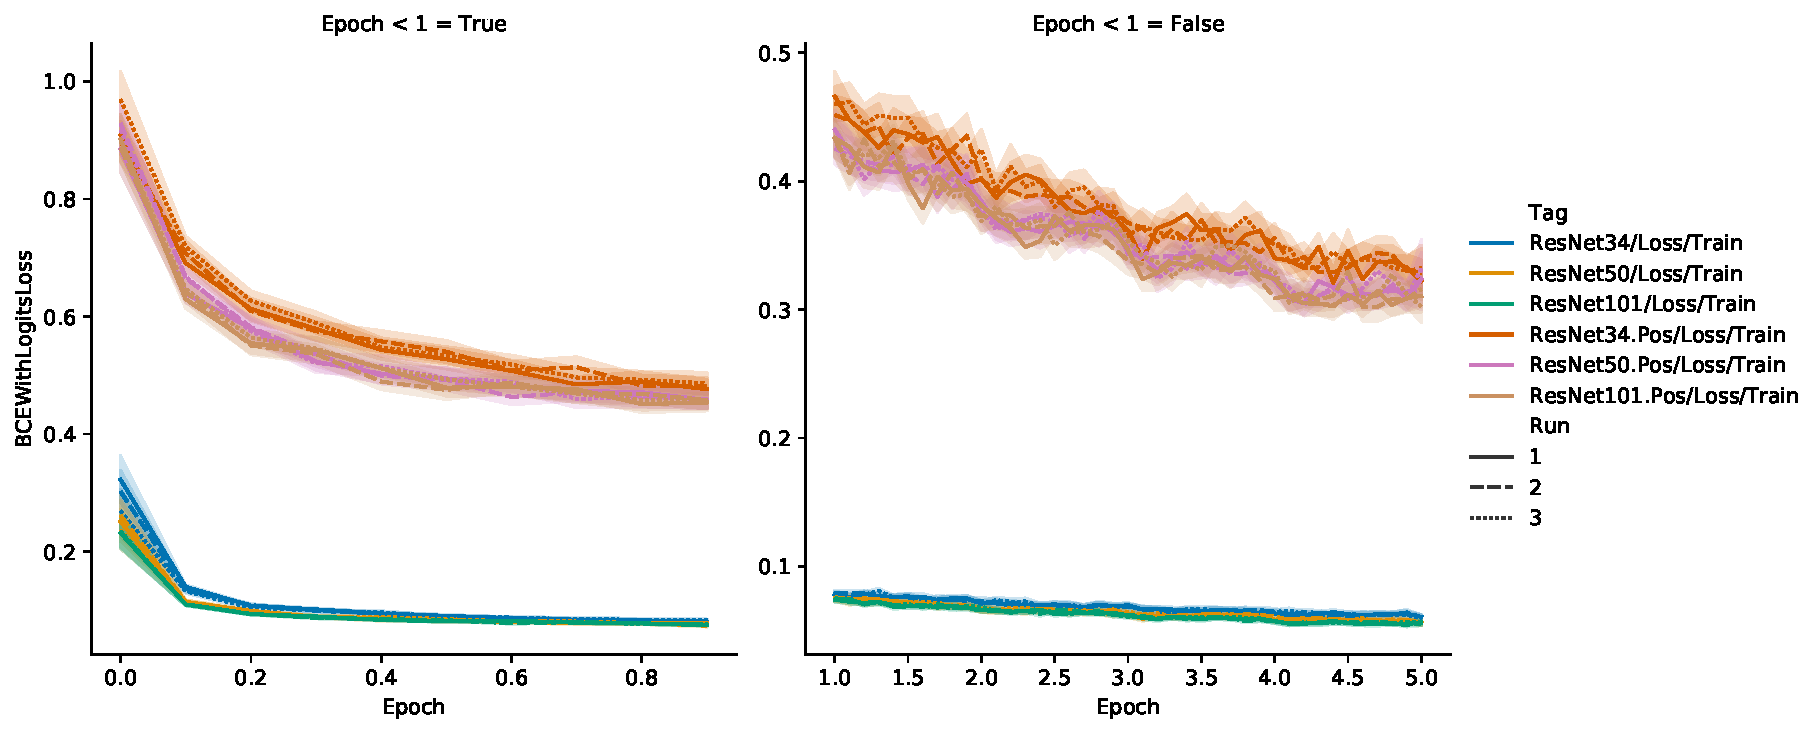
\includegraphics[width=4.8in]{fig/train_loss_epoch}
    \caption{Training loss over epoch for ResNet-[34,50,101], three runs each. Shaded region represents 95\% confidence interval over 0.1 epoch bins.}
    \label{fig:train_loss}
\end{figure}

\begin{figure}[htbp]
    \centering
    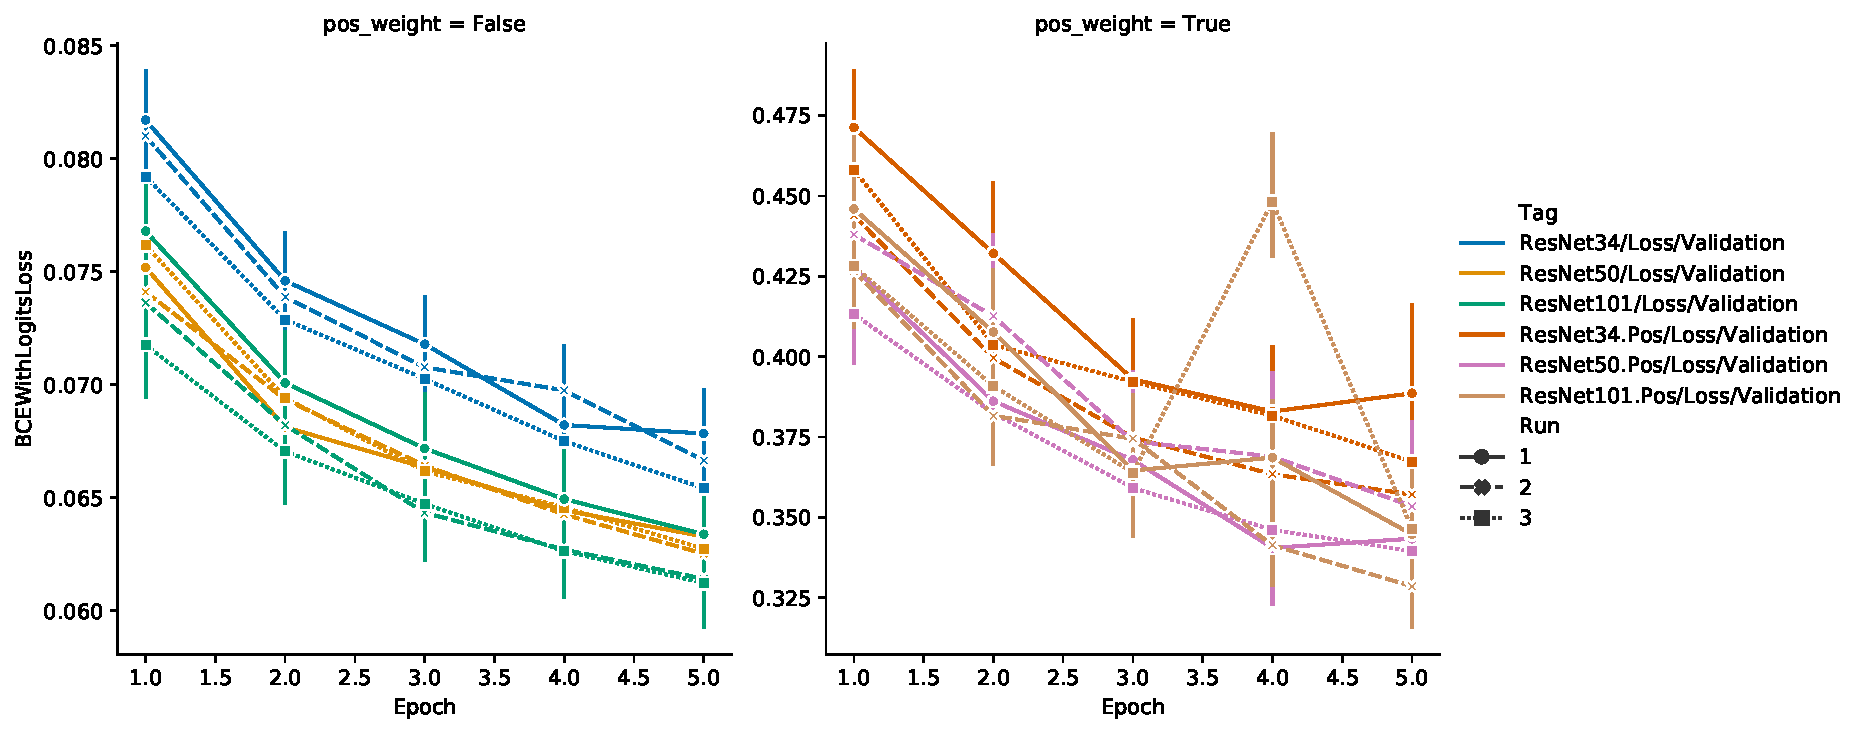
\includegraphics[width=4.8in]{fig/val_loss_epoch}
    \caption{Validation loss after training epoch for ResNet-[34,50,101], three runs each. Bars represent 95\% confidence interval over the entire validation dataset.}
    \label{fig:val_loss}
\end{figure}

The training and validation losses can be found in Fig.~\ref{fig:train_loss} and Fig.~\ref{fig:val_loss}.
A best-of summary for our models with comparisons to the Kaggle Top 3 leaderboard solutions can be found in Tab.~\ref{tab:result_summary}.
Our submissions were submitted after the challenge deadline, therefore estimated leaderboard positions were derived from submissions with scores nearest to ours.

\begin{table}[htbp]
    \centering
    \tabcolsep=0.11cm
    \caption{Experiment result summary and comparison with scores obtained by top three Kaggle competition winners.}
    \label{tab:result_summary}
    \begin{tabular}{|c|c|c|c|c|c|}
        \hline
        Model & Pos & Run & Validation Loss & Kaggle Score & Est. Leaderboard \\ \hline
        \multirow{2}{*}{ResNet-34}  & N & 3 & 0.001245 & 0.80829 & 421 \\
                                   & Y & 3 & 0.079299 & 0.64680 & 412 \\
        \multirow{2}{*}{ResNet-50}  & N & 1 & 0.019656 & 0.97402 & 424 \\
                                   & Y & 1 & 0.024243 & 0.71733 & 421 \\
        \multirow{2}{*}{ResNet-101} & N & 3 & 0.000912 & 0.78709 & 421 \\
                                   & Y & 2 & 0.030089 & 0.77097 & 421 \\
        \hline \hline
        \multicolumn{4}{|c|}{Kaggle Team Name} & Kaggle Score & Leaderboard  \\ \hline
        \multicolumn{4}{|c|}{SeuTao~\cite{kaggle/seutao}} & 0.04383 & 1 \\
        \multicolumn{4}{|c|}{NoBrainer~\cite{kaggle/nobrainer}} & 0.04484 & 2 \\
        \multicolumn{4}{|c|}{takuoko~\cite{kaggle/takuoko}} & 0.04510 & 3 \\ \hline
        
    \end{tabular}
\end{table}

The "Kaggle Score" evaluation was performed using a \emph{weighted multi-label logarithmic} loss applied to the test dataset submission.
In an effort to prevent competitors from taking advantage of the competition, the weights per label were not provided to contestants.
As the test dataset labels were not released, submitting our predictions to Kaggle was the only way to derive this metric.

Our model with the best score was \textbf{ResNet-34} with \texttt{pos\_weight} accounting for the dataset label sparsity.
This result suggests that ResNet-50 and ResNet-101 architectures were overfitting to the labelled data set, and did not generalize well to the unlabelled test set.
Additionally, all submissions that used \texttt{pos\_weight} outperformed submissions using the same model architecture but did not account for the label sparsity in the dataset.

Our best approach, compared to the competition submissions, would have achieved an approximate rank of 412 on the competition leaderboard.
However, the top 347 positions attained a score $< 0.1$, suggesting a large attainable improvement in test set performance.

\section{Discussion \& Future Work}
The top 12 teams from the leaderboard were bound by the competition guidelines to submit a summary of their neural network architecture, including training method, and feature selection/engineering methods.
Additionally, all their source code and configurations for executing and generating their submission file were made open source.
All 12 gold medalists used a windowing approach to convert the raw CT scan into a multi-channel image before extracting image features using a convolutional neural network.

Our approach evaluated DICOM CT scans one at a time, using the raw pixel data and windowing pre-processing only.
However, the high ranking Kaggle submissions exploited additional ID tags provided in the DICOM meta.
Using various configurations of the meta \texttt{Patient}, \texttt{Series}, and \texttt{Study} ID tags, competitors were able to create sequences of DICOM files.
The representation of the DICOM scans as sequences of data, rather than individual DICOM scans as isolated samples, was the key missing insight for attaining competitiveness in this challenge.
Our original intention behind not taking advantage of these tags was for our algorithm to maximize generalizeability using pixel data only.
For future competitions, our approaches should incorporate all meaningful meta data to better facilitate the challenge task.

Another unexplored approach is to train a CT scan encoder network and classify on the bottleneck learned feature vectors.
No ranked submissions used an encoder network as part of their deep learning pipeline, opting instead for convolutional feature extraction to recurrent neural network classification only.

\section{Conclusion}
To improve the speed for diagnosing ICH, we presented an algorithm to detect five different ICH sub-categories from DICOM files containing 2D CT scans of brain slices.
We presented an overview of the windowing approaches for brain ICH detection and a method using \texttt{BCEWithLogitsLoss} with \texttt{pos\_weight} for handling dataset label imbalance in a multi-label classification task.
We compared our results using three different ResNet architectures with the Kaggle competition winners and acknowledged the key missing insight of utilizing additional tags in the DICOM files to create sequences of CT scans.


\bibliographystyle{splncs04}
\bibliography{main}

\end{document}
